%seed - 34653286191

\documentclass[12pt]{article}

\usepackage[margin=0.5in]{geometry}
\usepackage{amsmath}
\usepackage{amsfonts}
\usepackage{amssymb}
\usepackage{graphicx}
\usepackage{tikz}
\usepackage{tcolorbox}
\usepackage[shortlabels]{enumitem}
\usepackage{ifthen}
\usepackage{xcolor}
\usepackage{tasks}
\usepackage{pgfplots}

% change this value to produce answer keys for exams
\newboolean{make_key}
\setboolean{make_key}{false}
\newcommand{\version}{}
% declarations for the different parts of the exam
\newtcolorbox{instructionbox}{
	colback = gray!25!white, 
	colframe = black!50!white, 
	boxrule = 0.4pt, 
	arc = 0pt
}

\newcommand{\iskey}[1]{\ifthenelse{\boolean{make_key}}{{\color{red}#1}}{}}

\begin{document}

% remove default page numbers
\pagestyle{empty}

% show the title information and student name
\noindent Not a real exam Version {\version} \hfill Name: \rule{6cm}{0.15mm} \vspace{2mm}

% show the instructions for the exam
\begin{instructionbox}
    \textbf{Instructions:} This is just a test of the emergency exam broadcast system.
    If it were a real exam, this note would be followed by instructions on how to complete
\end{instructionbox}

Is this the real life?
Is this just fantasy?

\begin{enumerate}

\item Here is a histogram: \\[4mm]
  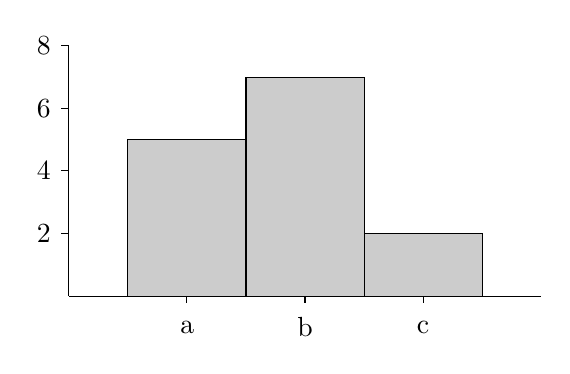
\begin{tikzpicture}[scale=1.5, yscale = 0.26485714285714285]
  \draw [thin, black] (0,0)--(4,0);
  \draw [thin, black] (0,0)--(0,8);
  \foreach \y in {2,4,6,8} {
    \draw[-] (0, \y)--(-2pt, \y) node[left] {$\y$};
  }
  \foreach \x/\l in {1/a,2/b,3/c} {
    \draw [-] (\x, 0)--(\x,-6pt) (\x, -1 )node {\l};
  }
  \foreach \x/\y in {1/5,2/7,3/2} {
    \draw [black, fill=black!20!white] (\x-0.5,0) rectangle (\x+0.5,\y);
  }
\end{tikzpicture}



\item This is a dot plot: \\[4mm]

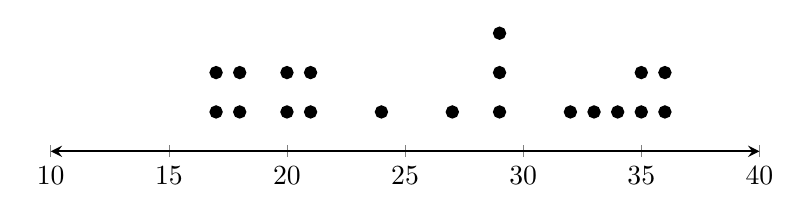
\begin{tikzpicture}
  \begin{axis}[axis lines=center, axis y line=none,
     x=3mm, y=5mm, xtick distance=5,
     axis line style={stealth-stealth, thick},
     xmin=10, xmax=40, ymin=0, ymax=3]
     \addplot [only marks, color=black, thick] coordinates { (17,1) (17,2) (18,1) (18,2) (20,1) (20,2) (21,1) (21,2) (24,1) (27,1) (29,1) (29,2) (29,3) (32,1) (33,1) (34,1) (35,1) (35,2) (36,1) (36,2)  };
  \end{axis}
\end{tikzpicture}



\item Find the class width of the set: 10, 17, 18, 24, 27, 63, 64, 75 \\[4cm]


\item (2 pts) 
Solve the inequality $ \displaystyle \frac{3.0}{x - 3} \geq \frac{1.0}{x + 1}$: \\[4mm]
\iskey{$ \displaystyle 3.0 x - 9.0 \geq 1.0 x + 1.0$}
\iskey{$\left[-3.0, -1\right) \cup \left(3, \infty\right)$}

\item (2 pts) Solve the polynomial equation: $ x^{2} + x = 0 $. \\[4mm]
\iskey{
    \begin{tabular}{ccl}
        $x^{2} + x$ & $=$ & $(x + 1)(x)$ \\[2mm]
        & $\Rightarrow$ & $x \in \left\{ \mathtt{\text{-1, 0}} \right\}$ \\
    \end{tabular}
}\item (2 pts) Solve the inequality $ \displaystyle \frac{1.0}{x + 1} \geq \frac{3.0}{x + 2}$: \\[4mm]
\iskey{$ \displaystyle 1.0 x + 1.0 \geq 3.0 x + 6.0$}
\iskey{$\left(-\infty, -2\right) \cup \left(-1, -0.5\right]$}


\vspace{3cm}


\item (4 pts) Solve the polynomial equation: $ 2 x^{2} + 3 x + 12 = 0 $. \\[4mm]

\iskey{
    $\displaystyle 2 x^{2} + 3 x = -12 $ \\[4mm]
    $\displaystyle x^{2} + \frac{3 x}{2} = -6 $ \\[4mm]
    $\displaystyle x^{2} + \frac{3 x}{2} + \frac{9}{16} = - \frac{87}{16} $ \\[4mm]
    $\displaystyle \left(x + \frac{3}{4}\right)^{2} = - \frac{87}{16} $ \\[4mm]
    $\displaystyle \left(x + \frac{3}{4}\right)^{2} = - \frac{87}{16} $ \\[4mm]
    $\displaystyle x + \frac{3}{4} = \pm \frac{\sqrt{87} i}{4} $ \\[4mm]

    $\displaystyle x \in \left\{ - \frac{3}{4} - \frac{\sqrt{87} i}{4}, - \frac{3}{4} + \frac{\sqrt{87} i}{4} \right\}$
}

\end{enumerate}
\end{document}